%%%% PROCESAR con PdfLaTeX !!!!!


\documentclass[12pt]{book}
\usepackage{geometry}\geometry{top=2cm,bottom=2cm,left=3cm,right=3cm}
\usepackage{amssymb}
\usepackage{amsmath}
\usepackage{graphicx}
\usepackage{txfonts}




\begin{document}
\thispagestyle{empty}

\begin {center}

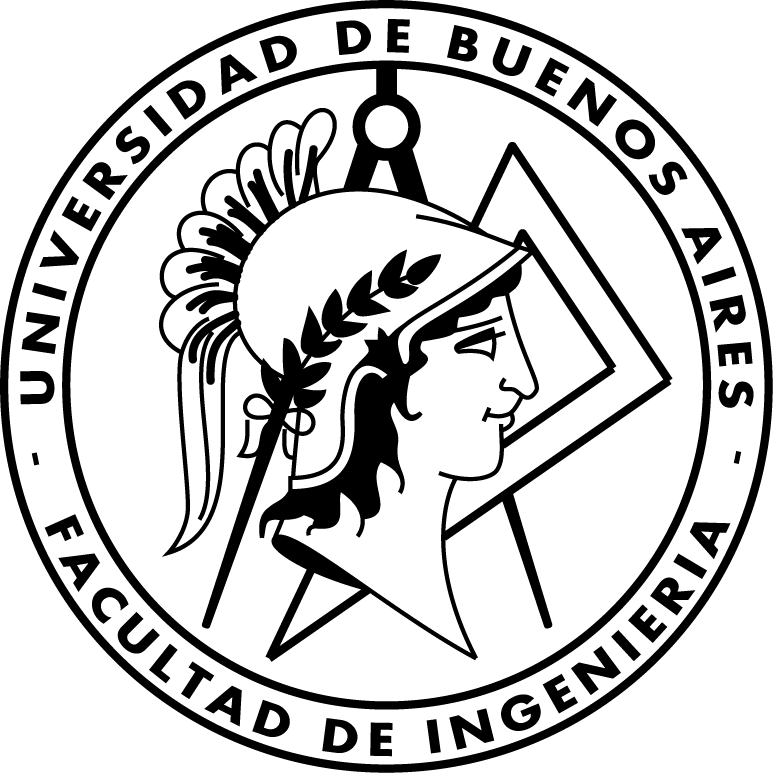
\includegraphics[scale=.4]{Logo-fiuba_big.png}

\medskip
UNIVERSIDAD DE BUENOS AIRES

Facultad de Ingenier\'ia

Departamento de Computaci\'on


\vspace{3cm}


\textbf{\large Elementos de probabilidad}

\vspace{2cm}


Este es un modesto aporte para los alumnos de la f\'acultad de ingenier\'ia  de la UBA de las carreras de licenciatura en an\'alsis de sistemas e ingenier\'ia inform\'atica.
De ninguna man\'era pretende ser una gu\'ia de estudio, ni remplaza las clases presenciales, el material oficial de la catedra esta disponible en el web site de la m\'ateria.
\\
https://campus.fi.uba.ar/course/view.php?id=1429
\end {center}


\vspace{2.5cm}

\noindent Autor:\,	Isaac Edgar Camacho Ocampo
 
\noindent Carrera:\,	Licenciatura en An\'alisis de sistemas

\vspace{1cm}

\vspace{1cm}

\noindent Buenos Aires, 2019

\newpage


\tableofcontents

\tableofcontents
\chapter{Introducción}
En el mundo real existen fenomenos que podemos conocer atravez de la experiencia, y la ciencia ha tratado a lo largo d ela historia de predecir tales acontecimientos, por ejemplo una tormenta una sequia etc. 
\\
Debido a la complejidad de la realidad es comun que los cientificos trabajen con simplificaciones que llamaremos modelos, que utilizamos para trabajar, es decir que trataremos de reproducir fenomenos y trataremos de predecir el resultado.
\\
Existen dos tipos de experimentos:
\begin{itemize}
\item Deterministicos: cuando bajo las mismas condiciones iniciales, se obtienen iguales resultados y de esto se encarga la fisica, por ejemplo con la ecuacion horaria $x_0 = x_i + v_0 t$

\item Estocasticos o aleatorios: Cuando bajo las mismas condiciones iniciales se obtienen varios resultados, por ejemplo \textbf{determinar la cantidad de lluvia en una zona} de esto se ocupa la Probabilidad.
\end{itemize}
\section{¿Que es la probabilidad?}
La misma nace con los juegos de azar, intuitivamente la podemos definir como:
\textbf{La probabilidad es el grado de certeza de que ocurrira un determinado resultado en un experimento aleatorio dado, cuanto mayor sea la probabilidad, mayor es el grado de certeza de que ocurrira dicho resultado} en otras palabras es la chance de que salga uno u otro resultado.
\\
por ejemplo:
\begin{itemize}
\item Que chance tengo de sacarme un 8 en un examen?
\item Que chance tengo de acertar la loteria?
\item que chances hay en sacar poker de ases?
\end{itemize}



\section{Estado del arte}
\chapter{Fundamentos teóricos}
\section{Teoría clásica}
\subsection{Definición de variables}
\subsection{Pruebas y refutaciones}
\section{Hipótesis}
\chapter{Resultados}
\section{Simulación de resultados}
\subsection{Suposiciones}
\subsection{Modelos}
\section{Resultados preliminares}
\section{Resultados postprocesados}
\subsection{Valores atípicos}
\subsection{Correlaciones}
\chapter{Conclusiones}
\end{document}
